\documentclass[12pt, a4paper]{article}

\usepackage[utf8]{inputenc}
\usepackage[brazil]{babel}

\usepackage[section]{placeins}

\usepackage[lmargin=2cm, rmargin=2cm, tmargin=2cm, bmargin=2cm]{geometry}

\usepackage{graphicx, amsmath, amssymb, graphicx, enumerate, , hyperref, color, libertine, listings, sectsty, pdfcomment, parskip}

\newcommand{\HRule}{\rule{\linewidth}{1pt}}

\sectionfont{\LARGE}
\subsectionfont{\Large}
\subsubsectionfont{\large}

\newif\ifxetexorluatex
\ifxetex
  \xetexorluatextrue
\else
  \ifluatex
    \xetexorluatextrue
  \else
    \xetexorluatexfalse
  \fi
\fi

\ifxetexorluatex%
  \usepackage{fontspec}
  \usepackage{libertine} % or use \setmainfont to choose any font on your system
  \newfontfamily\quotefont[Ligatures=TeX]{Linux Libertine O} % selects Libertine as the quote font
\else
  \usepackage[utf8]{inputenc}
  \usepackage[T1]{fontenc}
  \usepackage{libertine} % or any other font package
  \newcommand*\quotefont{\fontfamily{LinuxLibertineT-LF}} % selects Libertine as the quote font
\fi

\begin{document}

\begin{titlepage}
\begin{center}

\textsc{\large Universidade Federal de Santa Catarina}\\[1cm]

\includegraphics[width=0.3\textwidth]{ufsc}\\[1.5cm]

\textsc{\LARGE \bfseries Teoria da Computação \\ [0.8cm]}

\textsc{\LARGE \bfseries Problema da Correspondência de Post \\ [3cm]}


\begin{Large}
\textbf{Estudante}:
\begin{tabular}{|c}
Luc$\lambda$s Tonussi 12106577\\
\end{tabular} \\[0.5cm]
\end{Large}

\vfill

\begin{Large}
\textbf{Professora}:
\begin{tabular}{|c}
Jerusa Marchi \\
\end{tabular} \\[0.5cm]
\end{Large}

\vfill


\textbf{\today}

\end{center}
\end{titlepage}

\tableofcontents
\pagebreak

\listoffigures
\pagebreak

\listoftables
\pagebreak

\section{Recordando}

Conforme visto em sala, um problema \textbf{NP-Completo} é um problema que

\begin{enumerate}
  \item Está em \textbf{NP}.
  \item Todo problema $\Pi \in \text{\textbf{NP}}$ pode ser reduzido a ele em tempo polinomial.
\end{enumerate}

Também vimos que o problema da \textbf{Satisfazibilidade Booleana} (SAT) foi o primeiro problema a ser demonstrado \textbf{NP-Completo}. Há na literatura uma série de outros problemas provados \textbf{NP-Completos} \cite{sipser06}.

Em geral, a prova desta asserção consiste na redução de um problema reconhecidamente \textbf{NP-Completo} ao que se quer demonstrar.

\section{Trabalho 3}

Pesquisar e apresentar uma redução de um problema \textbf{NP-Completo} a outro. Alguns problemas clássicos são listados abaixo. Outros problemas podem ser encontrados \href{http://en.wikipedia.org/wiki/List_of_NP-complete_problems}{aqui!}.

\begin{itemize}
  \item Caminho Hamiltoniano. \cite{sipser06} {\color{red}\textbf{Grafos}}
  \item Caixeiro Viajante. {\color{red}\textbf{Grafos}}
  \item Caminho mais longo. {\color{red}\textbf{Grafos}}
  \item Clique. \cite{sipser06} {\color{red}\textbf{Grafos}}
  \item Mochila. {\color{red}\textbf{Grafos}}
  \item Cobertura Exata. {\color{red}\textbf{Grafos}}
  \item Vértices de Cobertura. \cite{sipser06} {\color{red}\textbf{Grafos}}
  \item Conjuntos Independentes. {\color{red}\textbf{Grafos}}
  \item Roteamento de Veículos. {\color{red}\textbf{Grafos}}
  \item Isomorismo em Grafos. {\color{red}\textbf{Grafos}}
  \item Caminho Rudrata. {\color{red}\textbf{Grafos}}
  \item Corte Balanceado. {\color{red}\textbf{Grafos}}
  \item Soma de Subconjuntos. \cite{sipser06} {\color{blue}\textbf{Conjuntos}}
\end{itemize}

\section{Pede-se}:

\begin{itemize}
  \item Enuncie os problemas envolvidos na redução.
  \item Esclareça o sentido da redução (problema fonte, problema destino).
  \item Apresente a redução.
\end{itemize}

\section{Pré-definições}

\begin{itemize}
  \item Consideremos o problema envolvendo o problema da soma dos subconjuntos no âmbito da aritmética com inteiros.
  \item Onde nesse problema nós temos uma coleção de números $x_1,x_2,x_3,...,x_k$.
  \item Onde também temos um objetivo (\textit{hint}) chamado $t$.
  \item Onde dada uma coleção de inteiros qualquer de tamanho $n$.
  \item Temos uma subcoleção dessa mesma, que se eu somar os elementos dessa irá dar $t$.
\end{itemize}

\subsection{Exemplo simples trivial}

$$A = {1,2,3,4,5,6,7}$$
$$t = 7$$
$$B = {3, 4}$$
$$SomaElementosB = 7$$

\subsection{Generalizando um pouco}

$$ \textit{SUBCONJUNTO-SOMA} = \lbrace \langle S, t \rangle | S = \lbrace  x_1,...,x_k \rbrace \text{ e para algum }$$

$$ \lbrace y_1,...,y_k \rbrace \subseteq \lbrace  x_1,...,x_k \rbrace \text{, nós temos } \Sigma{y_i} = t \rbrace \cite{sipser06}$$.

Note que: $x_1,...,x_k$ e $y_1,...,y_k$ são considerados a ser multi-listas e por isso, pode acontecer repetições dos elementos internos a elas (ie: $x_i == y_i$).

\section{Soma de Subconjuntos está em \textbf{NP}}

Por isso temos a intuição de que \textit{SUBCONJUNTO-SOMA} está em \textbf{NP}. Digamos que nós construíssemos uma máquina de turing $\textit{VERIFICADORA-SUBCONJUNTO-SOMA}_{tm}$ e essa máquina recebe como entrada $\langle \langle S, t \rangle , c \rangle$, que é um conjunto $S$ um alvo $t$ e $c$ um subconjunto que irá ser verificado pela máquina de turing. Ela irá verificar se a soma dos elementos de $c$ é igual a $t$.

$\textit{VERIFICADORA-SUBCONJUNTO-SOMA}_{tm} \leftarrow \langle \langle S, t \rangle , c \rangle$:

\begin{enumerate}
  \item Testa se c é uma coleção de números cuja soma é t.
  \item Testa se S contém todos os membros de c.
  \item Se (1 \& 2) passarem, $STATE_{accept}$ caso  contrário, $STATE_{reject}$
\end{enumerate}

\pagebreak

Poderíamos também usar uma máquina de turing que resolve isso não determinísticamente. Um adendo aqui que eu posso fazer é que essa máquina de turing agora é uma verificadora. O que acrescenta a ela algumas propriedades diferentes, a nova propriedade é a de receber uma entrada com a palavra (fita) e uma outra entrada com um dado específico, no meu caso um $t$. Porém o esquemático abaixo é só para esclarecimento didático. Na verdade eu prefiro pensar numa máquina de turing que recebe w e uma chute (um object, alvo, etc..) que funciona algoritmicamente do mesmo jeito. \cite{sipser06}

\begin{center}
  \begin{figure}[ht]
    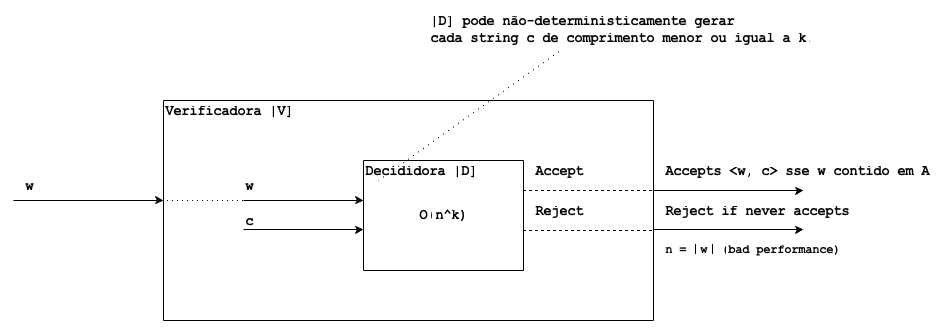
\includegraphics[scale=0.5]{verificadora.png} 
    \caption[Verificadora extende Decididora]{Verificadora extende Decididora para podermos trabalhar o problema da redução. Fonte: Própria}
  \end{figure}
\end{center}

$VERIFICADORA-ND-SUBCONJUNTO-SOMA_{tm} \leftarrow \langle S, t \rangle$:

\begin{enumerate}
  \item Não Determinísticamente Escolhe $c$, $c \in S$.
  \item Testa se c é uma coleção de números cuja soma é t.
  \item Se (2) passar, $STATE_{accept}$ caso  contrário, $STATE_{reject}$ 
\end{enumerate}

Observe que $\textit{SUBCONJUNTO-SOMA}^\complement$, não é membro de \textbf{NP}. E para abordar o problema menos ingênuamente, cria-se uma classe de complexidade algorítmica, chamada \textbf{coNP} a qual contêm as línguagens que são complemento das linguagens que estão \textbf{NP}. O livro do Sipser diz que nada pode-se afirmar sobre $\textbf{coNP } != \textbf{ NP}$ \cite{sipser06}. Porém no livro do Sudkamp página 484, ele prova o teorema 15.6.3 de que se existe ma línguagem \textbf{NP-completa} \textbf{L} com $\textbf{L}^\complement \in \textbf{NP}$, então $\textbf{NP } = \textbf{ coNP}$. e Anteriormente Sudkamp conclui que para o problema da satisfabilidade considerando o complemento do problema da satisfabilidade, pode-se examinar uma família de linguagens consistindo do complemento de todas as linguagens em NP. A família $\textbf{coNP } = {\lbrace \textbf{L}^\complement | \textbf{L} \in \textbf{NP} \rbrace}$. Apesar dessas incógnitas vamos prosseguir \textbf{confiando na idéia} $L(SUBCONJUNTO-SOMA) \in \textbf{NP}$ Para não haver confusão mais a frente. $\blacktriangleright$

\section{$SUBCONJUNTO-SOMA$ é \textbf{NP-completo}}

Basicamente a idéia é:

\begin{enumerate}
  \item Sabe-se que a línguagem $SUBCONJUNTO-SOMA$ está em \textbf{NP}.
  \item Prova-se que toda a línguagem \textbf{L} em \textbf{NP} pode ser redutível para tempo polinomial ao \textit{SUBCONJUNTO-SOMA}, diagonalizando uma fórmula booleana $F_{bool}$ que recebe o nome de \textit{Problema 3SAT} por ser uma linguagem formada dessa maneira $(x_1 \vee \neg x_2 \vee x_3) \wedge (x_2 \vee \neg \neg x_3 \vee \ldots) \wedge \ldots \wedge (\neg x_3 \vee \ldots \vee \ldots) \in \textbf{NP-Completo}$.
  \item Da forma que essa $F_{bool}$ pode ser redutível a \textit{SUBCONJUNTO-SOMA}
  \begin{enumerate}
    \item Acha-se um mapeamento de subconjuntos do problema \textit{SUBCONJUNTO-SOMA} que representam variáveis booleanas e cláusulas.
    \item Essas se formarão fórmulas que só podem usar $\wedge$, $\vee$, $\neg$ como operadores.
  \end{enumerate}
  \item Cada cláusula ie: ($x_1 \vee \neg x_2 \vee x_3$). Contém um certo valor da soma do alvo $t$, o qual impõe uma \textit{constraint} sobre o subconjunto a ter seus elementos somados.
  \item Prova-se por diagonalização de cantor que essa \textit{constraint} é a mesma que a sua correspondente cláusula  Ou seja podemos mapear. $\blacktriangleright$
\end{enumerate}.

\begin{quote}
  \flushright
    \begin{tabular}{|l}
    \textbf{Nota 01}: Eu menciono prova-se,\\
    tem-se, acha-se. Pois todo o sub-\\
    sídio está contido no livro do\\
    Sipser e/ou Sudkamp. os quais eu\\
    uso como base para explicar\\
  \end{tabular}
\end{quote}

\pagebreak
\subsection{Redução :: \textit{SUBCONJUNTO-SOMA} é \textbf{NP-completo}}

\begin{center}\begin{Huge}PROOF:\end{Huge}\end{center}

\textbf{Esclarecimentos iniciais}: o sentido da redução é do problema \textit{3SAT} $\Rightarrow$ Problema Fonte para \textit{SUBCONJUNTO-SOMA} $\Rightarrow$ Problema Destino.

\begin{enumerate}
  \item Sabe-se que o $\textit{SUBCONJUNTO-SOMA} \in \textbf{NP}$.
  \item Portanto vamos fazer $\textit{3SAT} \leqslant_{p} \textit{SUBCONJUNTO-SOMA}$.
  \item O objetivo é mapear uma fórmula booleana $F_{bool}$ de n variáveis para uma instância do problema do \textit{SUBCONJUNTO-SOMA}.
  \item Da forma que S deverá conter um par de números $y_i$, $z_i$ para cada variável $x_i$ em $F_{bool}$, $g_j$, $h_j$ para cada clausulá dessas: $(x_1 \vee \neg x_2 \vee x_3) \wedge (x_2 \vee \neg \neg x_3 \vee \ldots) \wedge \ldots \wedge (\neg x_3 \vee \ldots \vee \ldots)$


\begin{table}[h]\footnotesize
  \centering
\begin{tabular}{|c|c|c|c|c|c|c|c|c|c|c|}
	\hline
	 & 1 & 2 & 3 & 4 & $\cdots$ & \textit{l} & $c_1$ & $c_2$ & $\cdots$ & $c_k$ \\ 
	\hline 
	$y_1$ & 1 & 0 & 0 & 0 & $\cdots$ & 0 & 1 & 0 & $\cdots$ & 0 \\ 
	\hline 
	$z_1$ & 1 & 0 & 0 & 0 & $\cdots$ & 0 & 0 & 0 & $\cdots$ & 0 \\ 
	\hline 
	$y_2$ &  & 1 & 0 & 0 & $\cdots$ & 0 & 0 & 1 & $\cdots$ & 0 \\ 
	\hline 
	$z_2$ &  & 1 & 0 & 0 & $\cdots$ & 0 & 1 & 0 & $\cdots$ & 0 \\ 
	\hline 
	$y_3$ &  &  & 1 & 0 & $\cdots$ & 0 & 1 & 1 & $\cdots$ & 0 \\ 
	\hline 
	$z_3$ &  &  & 1 & 0 & $\cdots$ & 0 & 0 & 0 & $\cdots$ & 1 \\ 
	\hline 
	$\vdots$ &  &  &  & $\ddots$ & $\vdots$ & $\vdots$ &  &  & $\vdots$ & $\vdots$ \\ 
	\hline 
	$y_l$ &  &  &  &  &  & 1 & 0 & 0 & $\cdots$ & 0 \\ 
	\hline 
	$z_l$ &  &  &  &  &  & 1 & 0 & 0 & $\cdots$ & 0 \\ 
	\hline 
	$g_1$ &  &  &  &  &  &  & 1 & 0 & $\cdots$ & 0 \\ 
	\hline 
	$h_1$ &  &  &  &  &  &  & 1 & 0 & $\cdots$ & 0 \\ 
	\hline 
	$g_2$ &  &  &  &  &  &  &  & 1 & $\cdots$ & 0 \\ 
	\hline 
	$h_2$ &  &  &  &  &  &  &  & 1 & $\cdots$ & 0 \\ 
	\hline 
	$\vdots$ &  &  &  &  &  &  &  &  & $\ddots$ & $\vdots$ \\ 
	\hline 
	$g_k$ &  &  &  &  &  &  &  &  &  & 1 \\ 
	\hline 
	$h_k$ &  &  &  &  &  &  &  &  &  & 1 \\ 
	\hline 
	$t$ & 1 & 1 & 1 & 1 & $\cdots$ & 1 & 3 & 3 & $\cdots$ & 3 \\ 
	\hline
\end{tabular}
  \caption{Mapeamento \textit{3SAT} para \textit{SUBCONJUNTO-SOMA}}
\end{table}


\begin{quote}
  \flushright
    \begin{tabular}{|l}
\textbf{Nota 02}: Pode ser encontrada na\\ página 293 Sipser - Figura 7.57
  \end{tabular}
\end{quote}


\item Pode-se demonstrar que $F_{bool}$ é satisfazível \textbf{sse} algum subconjunto $c \in \langle S \rangle$, após seus elementos somados, a soma retornar t.

\item Agora, supondo que $F_{bool}$ é satisfazível mesmo.

\item Nós construímos um subconjunto vindo de $\langle S \rangle$.

\item Selecionamos $y_i$ se $x_i$ se retornar \textit{VERDADEIRO} e também $z_i$ se $x_i$ returna \textit{FALSO}.

\item Após o mapeamento, se somarmos as colunas, vamos completando 1's para os primeiros \textit{l} digitos. Pois selecionamos cada par do mapeamento ($y_i$ , $z_i$).

\item Cada um dos k's últimos digitos, é um número entre 1 e 3. Por causa que cada cláusula é satisfeita e também contém entre 1 e 3 incógnitas (ie: $(x_1 \vee \neg x_2 \vee x_3$).

\item Agora selecionando satisfazíveis g's e h's para mapear até k digitos (de 1 à 3) a máquina de turing pode atingir o alvo \textit{t}.

\item Para se ter 1 em cada $coluna[l]$ precisamos deu mais uma constrainte: $y_i \bigoplus z_i$ simplesmente para podermos atingir a satisfazibilidade: se o subconjunto $c$ contém $y_i$ o mapeamento marca $x_i \Rightarrow \textbf{VERDADE}$ caso contrário $x_i \rightarrow \textbf{FALSO}$

\item Para a $coluna[c]$ devemos ter mais uma constraint: pois deve haver espaço para a propagação dos carrys da $coluna[l]$ (que virão de $y_i$ ou $z_i$ mas não dos dois ao mesmo tempo, lembra que é xor) que irá propagar pelo menos 1 então os parzinhos ordenados precisam mapear até no máximo 2 na linha de $t$.

\item Se $y_i$ propaga o carry então $x_i = c_j  \wedge x_i \Rightarrow \textit{VERDADE}$.

\item Se $z_i$ propaga o carry então ${x_i}^\complement = c_j \wedge x_i \Rightarrow \textit{FALSO}$.

\item Nesse ponto se passaram as constraint: Temos $c_j$ satisfeito. e por sua vez $F_{bool}$ também. $\blacktriangleright$

\begin{quote}
  \flushright
    \begin{tabular}{|l}
\textbf{Nota 03}: Estou usando '$\Rightarrow$' \\ como símbolo de mapeamento.
  \end{tabular}
\end{quote}

\end{enumerate}

\section{Gran Finale}

Para o gran finale nós devemos ter certeza de que a redução pode ser feita em tempo polinomial. Analizando a tabela nós olhamos para k's digitos e l's digitos vindos da abstração binária de \textit{SUBCONJUNTO-SOMA} pode-se observar que ela contém ${(k + l)}^2$ e cada entrada pode ser calculada para alguma línguagem $F_{bool}$. Então o tempo total é $O(n^2)$.

\begin{quote}
  \flushright
    \begin{tabular}{|l}
				\textbf{Nota 04}: Para mostrar que ${(k + l)}^2$ é\\
				bigO de $n^2$ (f(n) mais justo possível) basta\\
				pegar $ k + l = t $. $t^2 Oc*{n}^2$ para $t=n>0;$\\
				$n_0=0; c>0;$ a volta segue o mesmo raciocínio.\\
  \end{tabular}
\end{quote}


A definição diz que A é poly-time redutível à B se A é redutível à B e o tempo para a redução é limitado por O($n^k$). Se A é $A \leqslant_{p} B$ e B é \textbf{NP} então A está em \textbf{NP}. Pode-se chegar a uma conclusão importânte que se uma línguagem A é \textbf{NP-complete} \textbf{sse}. \cite{sipser06}

\begin{enumerate}
  \item $A \in \textbf{ NP}$
  \item Para qualquer linguagem $L \in \textbf{ NP}$, onde $L \leqslant_{p} A$.
\end{enumerate}

Se A é \textbf{NP-complete} e $A \in \textbf{ P}$ então $\textbf{NP } \leqslant \textbf{ P}$. Então \textbf{P=NP?}. Mas o que se sabe é que não temos linguagem em  $\textbf{NPC } \in \textbf{ P}$ so, $\textbf{P } \neq \textbf{ NP}$. Se é conhecido como sendo \textbf{NPC} e se nós queremos mostrar que B é \textbf{NPC}, nós "podemos" fazer isso, mostrando uma redução em tempo polinomial (\textit{poly time reduction}) de \textbf{A} para \textbf{B} ao passo que $B \in NP$ também. O problema é que temos que saber que A é NP-Complete o que é uma grande dor de cabeça. E \textbf{SAT} é historicamente um deles. $\blacksquare$

O caso foi simplesmente particionar o problema em muitas cláusulas lógicas pequenas que torna possível o mapeamento de $\textit{3SAT} \leqslant_{p} \textit{SUBCONJUNTO-SOMA}$. A princípio eu procurei entender como reduzir o problema da soma do subconjuntos para Partições que soluciona o problema em tempo pseudo polinomial com programação dinâmica, com a ideia de se particionar o conjunto em dois conjuntos $S_1$ e $S_2$. E a soma dos elementos de $S_1$ é equivalente a soma dos elementos de $S_2$. Porém eu não consegui entender, pois envolve programação dinâmica (que é tópico de inteligência artificial) e envolve heurística (que também é tópico de inteligência artificial).

Portanto tentei explicar com minhas palavras o que o livro do Sipser (pg 263, 292) trás para deduzir o problema \textit{3SAT} ao problema da soma dos subconjuntos, o qual me parece mais simples. Do ponto de vista que tentar forçar ou simplesmente escrever uma prova de redução de problemas nessas classes NP, NPC, NP-Hard, etc. É muito complicado, para pouca base matemática. Já foi complicado entender a explicação dele sobre a redução \textit{3SAT} para \textit{SUBCONJUNTOS-SOMA}.

\pagebreak
\begin{thebibliography}{9}

\bibitem {sipser06} Sipser, M. Introduction to the Theory of Computation (2nd Ed), Thomson Course Technology © 2006, ISBN-13: 978-0-534-95097-2, ISBN-10: 0-534-95097-3.

\bibitem {stk01} Computer Science, Stackexchange; Disponível em: \href{http://cs.stackexchange.com/questions/6111/how-can-i-reduce-subset-sum-to-partition}{http://cs.stackexchange.com/questions/6111/how-can-i-reduce-subset-sum-to-partition}, Acesso \today.


\end{thebibliography}
\end{document}
